\documentclass[10pt,a4paper,titlepage]{article}
\usepackage[utf8]{inputenc}
\usepackage{amsmath}
\usepackage{amsfonts}
\usepackage{amssymb}
\usepackage[ngerman]{babel}
\usepackage[pdftex]{graphicx}
\usepackage[vmargin=3cm, hmargin=2cm]{geometry}
\usepackage{tabularx}

\setlength{\parindent}{0pt}
\setlength{\parskip}{2pt}

\title{Entwurfsdokument}
\author{Simon Bischof \and Jan Haag \and Adrian Herrmann \and Lin Jin \and Tobias Schlumberger \and Matthias Schnetz}

\makeindex

\begin{document}

\thispagestyle {empty}
\vspace*{4cm}
\begin{center}
\begin {huge}
Entwurfsdokument\\
\end{huge}
Simon Bischof, Jan Haag, Adrian Herrmann, Lin Jin, Tobias Schlumberger, Matthias Schnetz\\
\vspace{3cm}
\begin{huge}
Praxis der Softwareentwicklung \\
Projekt 3:\\
Automatisches Pr\"{u}fen der Korrektheit von Programmen\\
Gruppe 1\\
\vspace{2cm}
\includegraphics[height=2cm]{images/Logo.pdf}\\[0.5cm]
\end{huge}
\begin{huge}
WS 2011/2012
\end{huge}
\end{center}
\newpage
\tableofcontents
\newpage

\section{Klassendiagramme}
\subsection{"Ubersicht}
Dieses Klassendiagramm zeigt die Grobstruktur der Anwendung. \\
\includegraphics[scale=0.8]{images/ClassOverview.pdf} \\
Die gesamte Architektur basiert auf dem Entwurfsmuster Model-View-Controller. Dies erm"oglicht uns einen flexiblen Programmentwurf, der eine sp"atere "Anderung oder Erweiterung erleichtert und eine Wiederverwendbarkeit der einzelnen Komponenten erm"oglicht. 
\begin{itemize}
\item Das \textbf{Modell} enth"alt die darzustellenden Daten, z.B die Zust"ande der Variablen w"ahrend der Programmausf"uhrung und die vom Benutzer gesetzten Breakpoints
\item Die \textbf{Pr"asentation/View} stellt die Daten aus dem Modell auf der Benutzeroberfl"ache dar und nimmt Benutzerinteraktionen entgegen
\item Um die Zusammenarbeit der ersten zwei Komponenten k"ummert sich die \textbf{Steuerung}. Au"serdem f"uhrt sie die Hauptaktionen (Parsen, Interpretieren, usw.) aus und bearbeitet die Eingaben des Benutzers \\\\
\end{itemize} 
\subsection{Feinstruktur der Komponenten}
\subsubsection{Programmstruktur} 
Dieses Klassendiagramm stellt mithilfe des Kompositum-Musters die Struktur des AST dar. \\\\
\includegraphics[scale=0.85]{images/AST.pdf}
\begin{itemize}
\item \textbf{Program} \\
Die Klasse \textbf{Program} stellt eine Funktion im Quelltext dar. \\\\
Attribute: \\
\textbf{program} \\
eine Instanz von sich selbst. Diese sind Unterprogramme, die aufgerufen werden k"onnen.\\
\textbf{statement} \\
eine Liste von Instanzen der Klasse \textbf{Statement}
\item \textbf{Statement} \\
Die abstrakte Klasse \textbf{Statement} steht f"ur eine Anweisung des Programms. Die Anweisungen sind eingeteilt in f"unf Klassen: \textbf{Conditional, Loop, Specification, Assignment} und \textbf{Expression}. \\\\
Attribut:\\
\textbf{line} \\
Zeile im Quelltext, in der sich die Instanz befindet\\\\
Methoden: \\
\textbf{getLine()} \\
gibt das Attribut \textbf{line} zur"uck \\
\textbf{\textit{accept(visitor: ProgramVisitor)}}\\
abstrakte Methode, die von den Unterklassen implementiert wird 
\item \textbf{Conditional} \\
Die Klasse \textbf{Conditional} steht f"ur eine bedingte Anweisung. \\\\
Attribut: \\
\textbf{program} \\
Unterprogramme, die bedingt ausgef"uhrt werden \\
\textbf{condition} \\
Bedingung, die "uberpr"uft wird 
\item \textbf{Loop} \\
Die Klasse \textbf{Loop} steht f"ur eine while-Anweisung. \\\\
Attribute: \\
\textbf{program} \\
Unterprogramme, die bedingt ausgef"uhrt werden \\
\textbf{condition} \\
Bedingung, die "uberpr"uft wird
\item \textbf{Specification} \\
Attribut: \\
\textbf{spec} \\
Ausdruck, der "uberpr"uft wird
\item \textbf{Assignment} \\
Die Klasse \textbf{Assignment} steht f"ur eine Zuweisung von Variablen. \\\\
Attribute: \\
\textbf{value} \\
der Wert, der zugewiesen wird\\
\textbf{identifier} \\
die Variable, der \textbf{value} zugewiesen wird 
\item \textbf{Expression} \\
Die abstrakte Klasse \textbf{Expression} steht f"ur einen beliebigen Ausdruck. \textbf{QuantifiedExpression, ArithmeticExpression, LogicalExpression, FunctionCall} und \textbf{VariableAccess} sind Unterklassen dieser Klasse.
\end{itemize}
\subsubsection{Besucherklassen}
\includegraphics[scale=0.7]{images/Besucher.pdf}
\subsubsection{Parser}
\includegraphics[scale=0.6]{images/Parser.pdf}
\subsubsection{Modell}
\includegraphics[scale=0.8]{images/Modell.pdf}
\subsubsection{Benutzeroberfl"ache}
\includegraphics[scale=0.85]{images/Gui.pdf}

\section{Verhaltensdiagramme}
\subsection{Aktivit"atsdiagramme}
\subsubsection{Parser/Type-Checker}
\includegraphics[scale=0.8]{images/AktivitaetParser.pdf}\newline
Beim Aufruf des Interpreters wird das Programm in mehreren Schritten geparst.
\begin{enumerate}
\item Der Programmtext wird als einzelner String dem Tokenizer "ubergeben.
\item Der Tokenizer trennt den String an den wichtigen Stellen und gibt ein Array von Tokens zur"uck.
\item Der Parser generiert bei syntaktisch korrekten Programmen daraus einen abstrakten Syntaxbaum (AST).
\item Bei Syntaxfehlern bricht der Parser mit einem Fehler ab.
\item Im Erfolgsfall "uberpr"uft der Typechecker die Korrektheit der Typen: Sind die Typen korrekt, gibt dieser den vom Parser generierten AST zur"uck, sonst beendet er sich mit einem Fehler.
\end{enumerate}
\subsubsection{Z3-Anbindung}
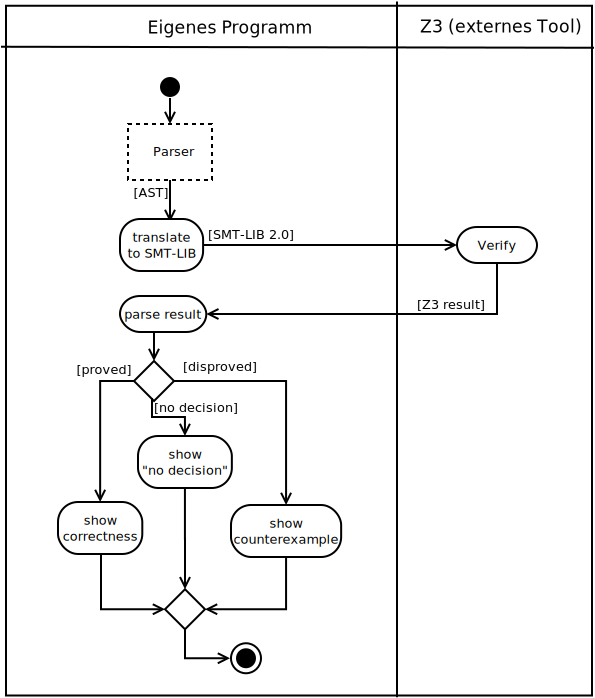
\includegraphics[scale=0.6]{images/AktivitaetSMTTranslator.pdf}\\
Zur "uberpr"ufung der Korrektheit des Programms wird Z3 benutzt. \\
\begin{enumerate}
\item Zuerst wird das Programm geparst (siehe Aktivit"atsdiagramm Parser/Type-Checker). 
\item Im Fehlerfall ist keine "Uberpr"ufung durch Z3 m"oglich. Im Erfolgsfall wird der durch den Parser generierte AST an den SMTLib-Translator gegeben. 
\item Der SMTLib-Translator "ubersetzt das Programm inklusive Spezifikation ins SMTLib-2.0-Format. Dieses bildet die Eingabe f"ur Z3.
\item Die von Z3 zur"uckgegebene Antwort wird vom Result-Parser analysiert. 
\item Meldet der Beweiser die Korrektheit des Programms oder konnte er keine Entscheidung treffen, wird dieses Ergebnis dem Benutzer bekannt gegeben. Falls der Beweiser das Programm falsifizieren konnte, wird dem Benutzer das Ergebnis zusammen mit einem m"oglichen Gegenbeispiel angezeigt.
\end{enumerate}
\subsection{Zustandsdiagramm}
Das folgende Zustandsdiagramm zeigt das Verhalten des Systems bei Benutzeraktionen. \\
\includegraphics[scale=0.9]{images/Zustand.pdf}\\
\begin{itemize}
\item Beim Starten des Programms geht dieses in den "`idle"'-Zustand. Hier l"auft der Interpreter nicht, und es ist kein Programmzustand gespeichert. Falls einer vorhanden ist, wird dieser beim Eintritt in den "`idle"'-Zustand gel"oscht.
\item Beim Ausw"ahlen von "`single step"' wird das Userprogramm geparst und ein Statement wird ausgef"uhrt, nachdem der Zustand "`single step"' betreten worden ist. Ist kein Statement mehr vorhanden, so beendet sich der Interpreter, das Programm geht zur"uck in den Zustand "`idle"'. Sonst wird nach Ausf"uhren des Statements das Programm pausiert, der Zustand "`paused"' wird eingenommen. 
\item Beim Eintritt in den "`paused"'-Zustand wird der Zustand des Userprogramms ausgegeben. W"ahrend der Pausierung l"auft der Interpreter nicht. In diesem Zustand stehen die gleichen M"oglichkeiten wie im "`idle"'-Zustand zu Verf"ugung, das Parsen bei Verlassen des Zustands entf"allt aber.
\item Wenn im "`idle"'-Zustand "`run to breakpoint"' aufgerufen wird, wird das Userprogramm geparst und das Programm geht in den Zustand "`run"'. Das Userprogramm wird solange ausgef"uhrt, bis es zu Ende ist (neuer Zustand: "`idle"') oder der Interpreter pausiert, ein Breakpoint getroffen oder eine Assertion falsifiziert wird. In diesen F"allen ist der neue Zustand "`paused"'.
\item In jedem Zustand au"ser "`idle"' ist es zus"atzlich m"oglich, das Userprogramm abzubrechen, wobei der Interpreter beendet wird und alle vorhandenen Variablen-Informationen gel"oscht werden. Das Programm geht danach in den Zustand "`idle"'.
\item In jedem Zustand kann das Programm durck einen Klick auf den Exit-Button beendet werden.
\end{itemize}
\newpage

\section{Syntax der While-Sprache}
\subsection{"Ubersicht der Schl"usselw"orter und Sonderzeichen}
\begin{ttfamily}
\begin{tabular}{| l  l |}
\hline
\hspace*{1.5cm}boolean & $\to$ type\_specifier\hspace*{2cm}\\\hline
\hspace*{1.5cm}else & $\to$ if\_statement\hspace*{2cm}\\\hline
\hspace*{1.5cm}false & $\to$ logical\_literal\\\hline
\hspace*{1.5cm}if & $\to$ if\_statement\\\hline
\hspace*{1.5cm}int & $\to$ type\_specifier\\\hline
\hspace*{1.5cm}return & $\to$ statement\\\hline
\hspace*{1.5cm}true & $\to$ logical\_literal\\\hline
\hspace*{1.5cm}while & $\to$ while\_statement\\\hline
\hspace*{1.5cm}0..9 & $\to$ integer\_literal\\\hline
\hspace*{1.5cm}a..z,A..Z,\_\hspace*{1cm} & $\to$ identifier\\\hline
\hspace*{1.5cm}\& & $\to$ mul\_expression\\\hline
\hspace*{1.5cm}| & $\to$ add\_expression\\\hline
\hspace*{1.5cm}! & $\to$ unary\_expression\\\hline
\hspace*{1.5cm}!= & $\to$ expression\\\hline
\hspace*{1.5cm}== & $\to$ expression\\\hline
\hspace*{1.5cm}< & $\to$ rel\_expression\\\hline
\hspace*{1.5cm}<= & $\to$ rel\_expression\\\hline
\hspace*{1.5cm}> & $\to$ rel\_expression\\\hline
\hspace*{1.5cm}>= & $\to$ rel\_expression\\\hline
\hspace*{1.5cm}+ & $\to$ add\_expression\\
 & $\to$ unary\_expression \\\hline
\hspace*{1.5cm}- & $\to$ add\_expression\\
 & $\to$ unary\_expression \\\hline
\hspace*{1.5cm}* & $\to$ mul\_expression\\\hline
\hspace*{1.5cm}/ & $\to$ mul\_expression\\\hline
\hspace*{1.5cm}\% & $\to$ mul\_expression\\\hline
\hspace*{1.5cm}, & $\to$ arglist \\
 & $\to$ parameter\_list \\
 & $\to$ variable\_declaration \\
 & $\to$ variable\_initializer\\\hline
\hspace*{1.5cm}; & $\to$ statement \\\hline
\hspace*{1.5cm}= & $\to$ variable\_declarator\\
 & $\to$ statement \\\hline
\hspace*{1.5cm}( & $\to$ bracket\_expression \\
 & $\to$ if\_statement \\
 & $\to$ while\_statement\\
 & $\to$ methode\_call \\
 & $\to$ methode\_declaration \hspace*{5cm}\\\hline
\hspace*{1.5cm}) & $\to$ bracket\_expression \\
 & $\to$ if\_statement \\
 & $\to$ while\_statement\\
 & $\to$ methode\_call \\
 & $\to$ methode\_declaration \\\hline
\hspace*{1.5cm}[ & $\to$ array\_access \\
 & $\to$ type \\\hline
\hspace*{1.5cm}] & $\to$ array\_access \\
 & $\to$ type \\\hline
\hspace*{1.5cm}\{ & $\to$ statement\_block \\
 & $\to$ variable\_initializer\\\hline
\hspace*{1.5cm}\} & $\to$ statement\_block \\
 & $\to$ variable\_initializer\\\hline
\hspace*{1.5cm}\# & $\to$ comment\\\hline
\end{tabular}
\end{ttfamily}

\subsection{Startsymbol}
\texttt{compilation\_unit}
\subsection{Produktionsregeln}
\begin{ttfamily}
\shorthandoff{"}
add\_expression ::= mul\_expression  \{ ( "|" $\mid$ "+" $\mid$ "-" ) mul\_expression \} \\\\
arglist ::=  expression \{ "," expression \}\\\\
array\_access ::= identifier "$[$" expression "$]$" \{ "$[$" expression "$]$" \} \\\\
bracket\_expression ::= "(" expression ")" \\
\hspace*{4.5cm}$\mid$ method\_call \\
\hspace*{4.5cm}$\mid$ array\_access \\
\hspace*{4.5cm}$\mid$ identifier \\
\hspace*{4.5cm}$\mid$ literal\_expression \\\\
comment ::= "\#" .* ( "\textbackslash n" $\mid$ "\textbackslash r" ) \\\\
compilation\_unit ::= \{ field\_declaration \}\\\\
expression ::= rel\_expression \{ ( "==" $\mid$ "!=" ) rel\_expression \}\\\\
field\_declaration ::= ( $[$ comment $]$ ( method\_declaration \\
\hspace*{7cm}$\mid$ statement ) )\\\\
identifier ::= "a..z,A..Z,\_" \{ "a..z,A..Z,\_,0..9" \}\\\\
if\_statement ::= "if" "(" expression ")" statement\_block $[$ "else" statement\_block $]$\\\\
integer\_literal ::= ( "0..9" \{ "0..9" \} )\\\\
literal\_expression ::= integer\_literal\\
\hspace*{4.5cm}$\mid$ logical\_literal \\\\
logical\_literal ::= "true" $\mid$ "false" \\\\
method\_call ::= identifier ( "(" $[$ arglist $]$ ")" )\\\\
method\_declaration ::= type identifier "(" $[$ parameter\_list $]$ ")" ( statement\_block )\\\\
mul\_expression ::= unary\_expression \{ ( "\&" $\mid$ "*" $\mid$ "/" $\mid$ "\%" ) 
unary\_expression \} \\\\
parameter ::= type identifier \\\\
parameter\_list ::= parameter \{ "," parameter \} \\\\
rel\_expression ::= add\_expression $[$ ( "<" $\mid$ "<=" $\mid$ ">" $\mid$ ">=" ) add\_expression $]$ \\\\
statement ::= variable\_declaration ";"\\
\hspace*{3cm}$\mid$ identifier "=" variable\_initializer ";"\\
\hspace*{3cm}$\mid$ ( expression ";" ) \\
\hspace*{3cm}$\mid$ ( if\_statement ) \\
\hspace*{3cm}$\mid$ ( while\_statement ) \\
\hspace*{3cm}$\mid$ ( "return" $[$ expression $]$ ";" ) \\\\
statement\_block ::= "\{" \{ statement \} "\}" \\\\
type ::= type\_specifier \{ "[" "]" \} \\\\
type\_specifier ::= "boolean" $\mid$ "int" \\\\
unary\_expression ::= $[$ ( "!" $\mid$ "+" $\mid$ "-" ) $]$ bracket\_expression \\\\
variable\_declaration ::= type identifier \{ "," identifier \} $[$ "=" variable\_initializer $]$ \\\\
variable\_initializer ::= expression \\
\hspace*{4.8cm}$\mid$ ( "\{" $[$ variable\_initializer \{ "," variable\_initializer \} $]$ "\}" ) \\\\
while\_statement ::= "while" "(" expression ")" statement\_block \\
\shorthandon{"}
\end{ttfamily}
\includegraphics[scale=0.73]{images/Grammar.pdf}

\end{document}

